\begin{frame}{Multistatic Networks are Growing}
    \begin{columns}
        \begin{column}{0.5\textwidth}
            Understanding global atmospheric dynamics requires \alert{global observations}! \\ ~ \\
        
            Multistatic networks are expanding across the globe 
            % {\setlength{\leftmargini}{1em} \begin{itemize} \footnotesize
            %     \item Established networks are expanding
            %     \item New networks are being built
            % \end{itemize}}
            \centering
            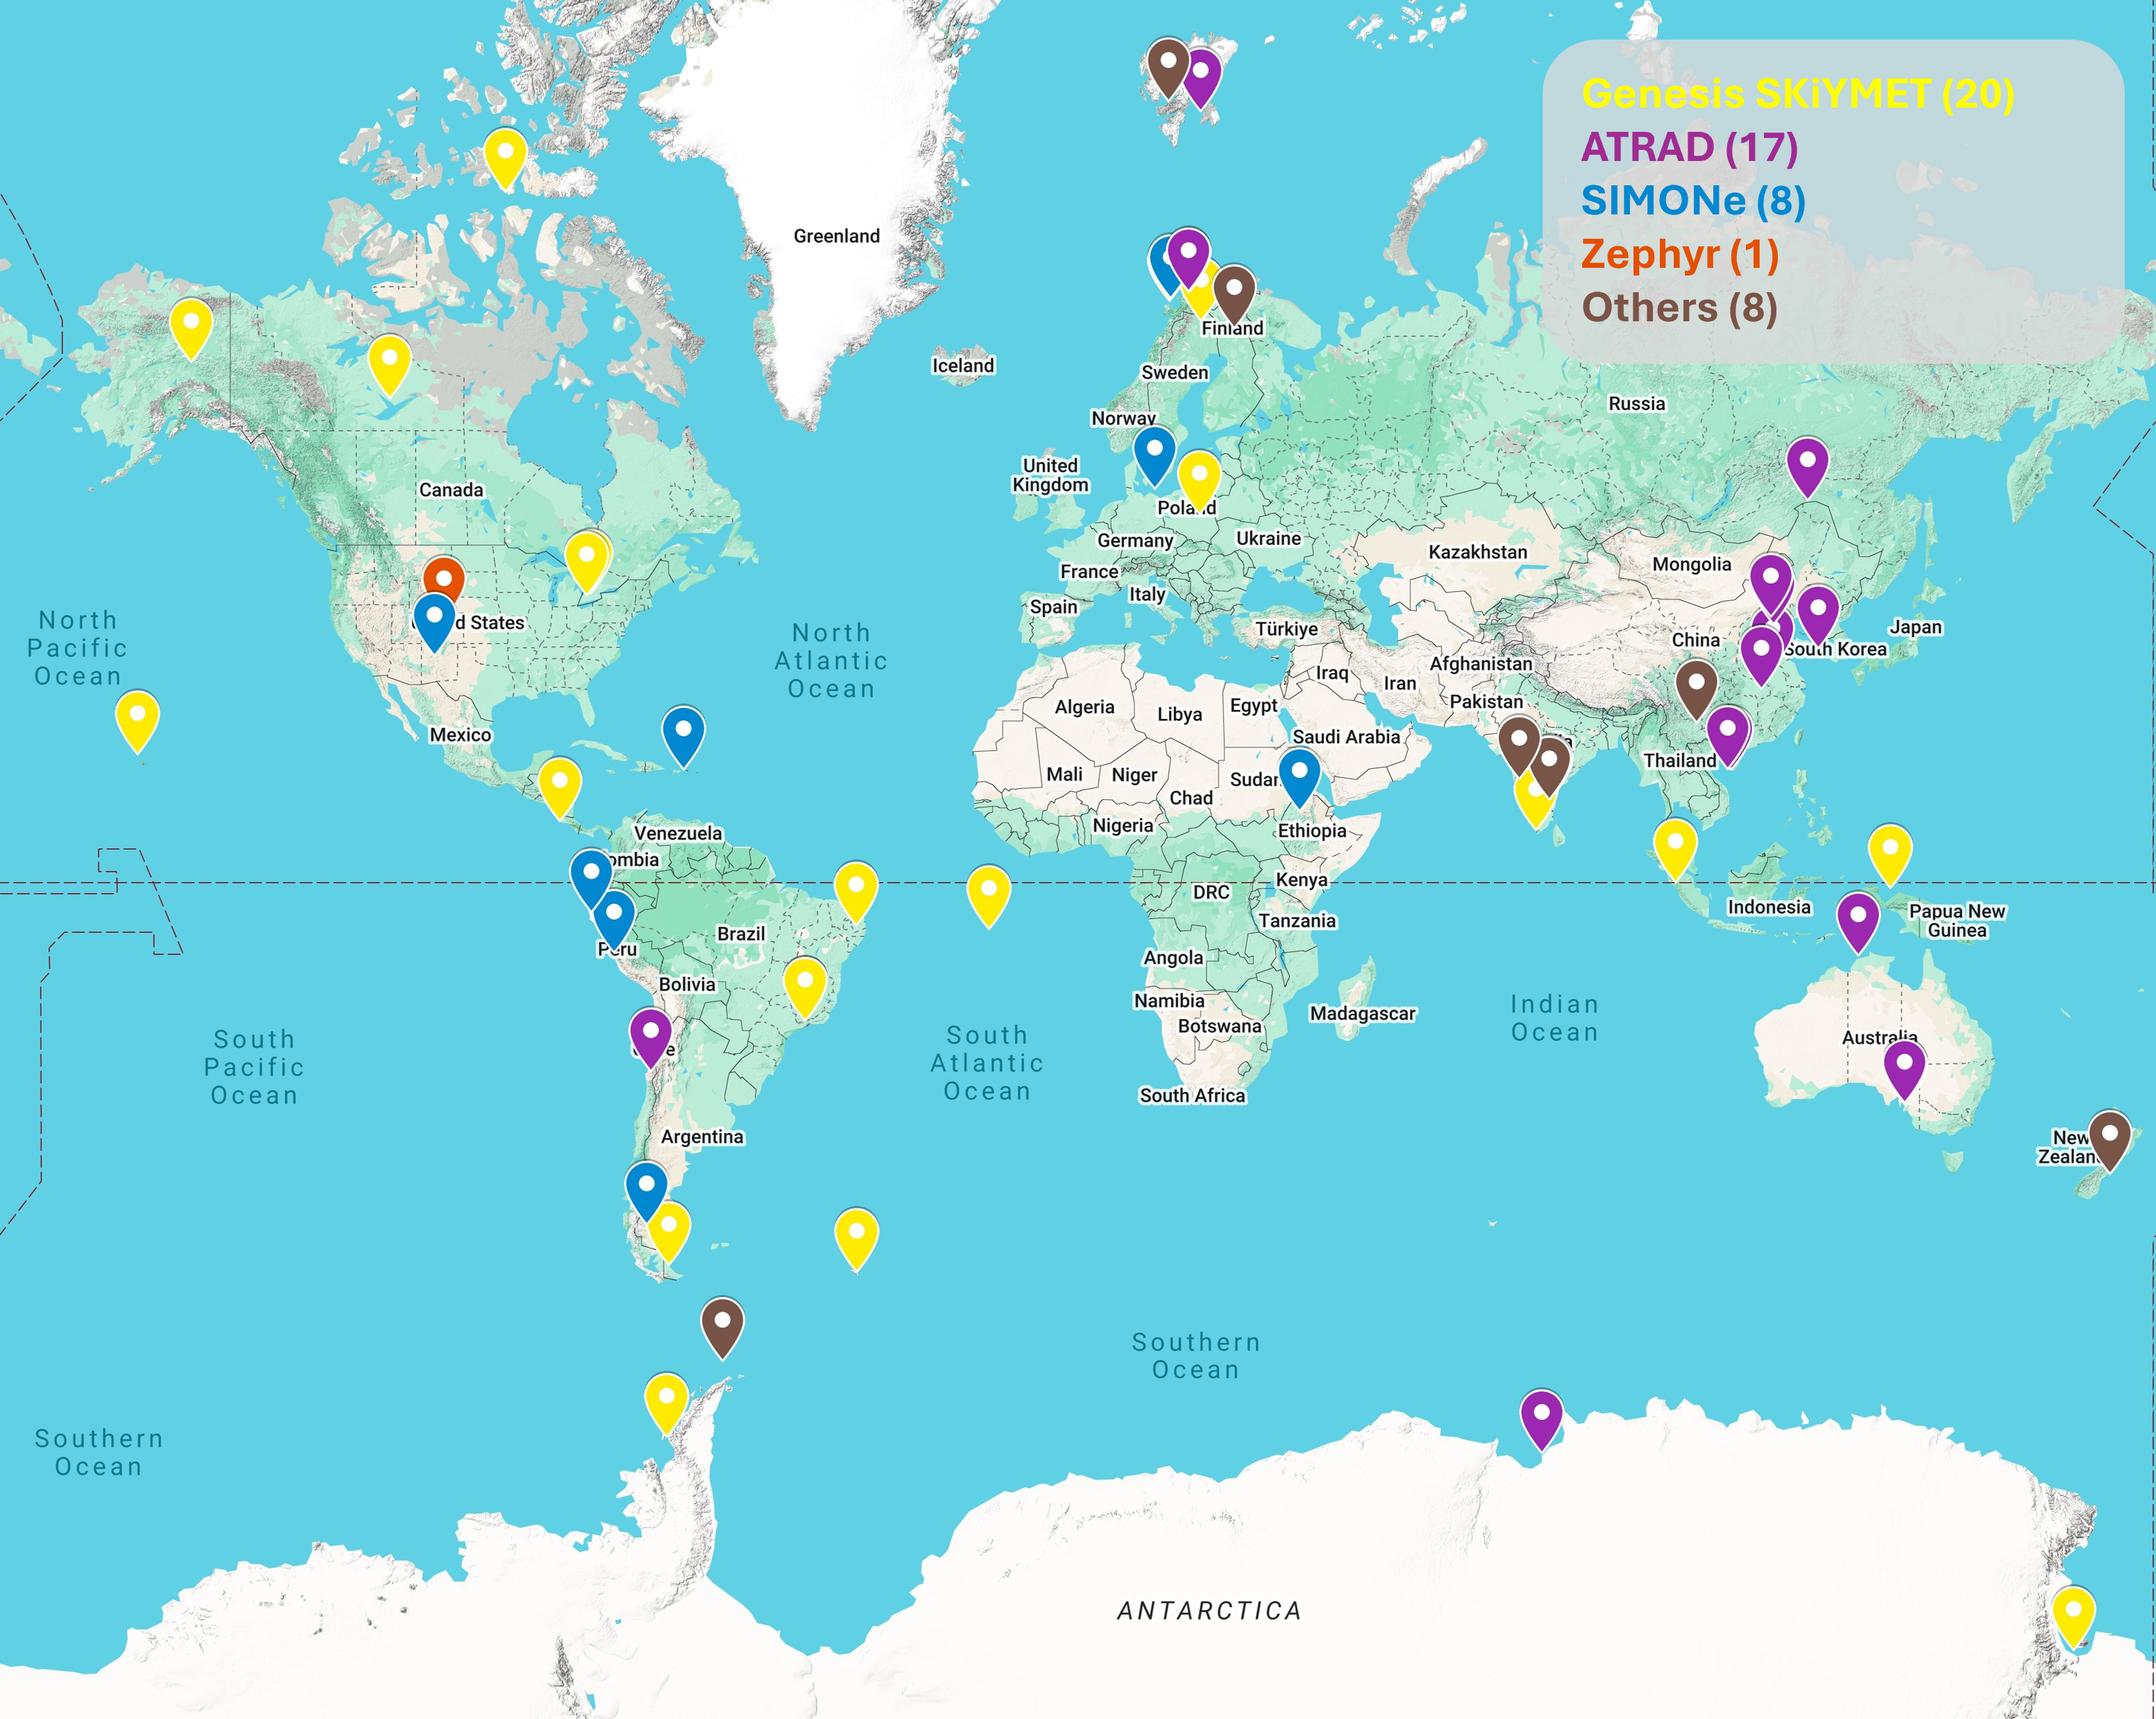
\includegraphics[width=0.7\linewidth]{img/smr_map.png}
        \end{column}
        \vrule{}
        \begin{column}{0.55\textwidth}
            \pause
            \uncover<+->{With limited resources, it is important to be able to answer:} 
            \begin{itemize}
                \item<+-> Best location for new \textcolor{blue}{\textbf{TX}} or \textcolor{red}{\textbf{RX}}? 
                \item<+-> Density of \textcolor{blue}{\textbf{TX}}/\textcolor{red}{\textbf{RX}} required?
                \item<+-> How many more meteors can we see?
                \item<+-> Best network configuration? Spacing, arrangement?
                \item<+-> \alert{What network improvements give the best science?}
            \end{itemize}
            \centering 
            \uncover<+->{\begin{tcolorbox}[width = \linewidth, center, boxrule=0pt,colback=yellow,arc=0pt,auto outer arc,left=0pt,right=0pt,boxsep=0pt]
                \centering
                No established tools can answer these questions
            \end{tcolorbox}}
        \end{column}
    \end{columns}
\end{frame} 

